\chapter{Analyse et conception}
\label{chap:analyse_conception}

\section{Introduction}

Ce chapitre présente la modélisation du système NetSentry : le diagramme de cas
d'utilisation, qui formalise les interactions entre les acteurs et le système, le
diagramme de séquence, qui détaille le déroulement complet d'un scan, et le modèle
conceptuel de données, qui structure les informations persistées en base.

\section{Diagramme de cas d'utilisation}

Le système NetSentry expose un seul rôle applicatif : un \textbf{administrateur IT}
authentifié, qui pilote le tableau de bord, déclenche les scans et traite les alertes.
Un second acteur, purement système, intervient également : le \textbf{planificateur
(cron)}, qui déclenche automatiquement les scans planifiés sans intervention humaine.

Toutes les actions accessibles à l'administrateur IT -- à l'exception de
l'authentification elle-même -- nécessitent une session valide : chacune d'elles inclut
donc (relation \texttt{«include»}) le cas d'utilisation \textbf{S'authentifier}, qui
repose sur la vérification des identifiants et l'émission d'un jeton JWT. C'est
également le cas des deux cas d'utilisation qui déclenchent un scan (\textit{Lancer un
scan manuel} et \textit{Exécuter un scan planifié}), qui incluent tous deux le
sous-comportement \textbf{Détecter les appareils (Nmap)}, commun aux deux modes de
déclenchement. La figure~\ref{fig:usecase} présente l'ensemble de ces cas d'utilisation
et de leurs relations.

\begin{sidewaysfigure}
    \centering
    
\includegraphics[height=0.88\textheight]{figuresChapitres/use_case.png}
    \caption{Diagramme de cas d'utilisation de NetSentry : l'authentification est
    incluse par l'ensemble des actions de l'administrateur IT}
    \label{fig:usecase}
\end{sidewaysfigure}

Comme le montre la figure~\ref{fig:usecase}, l'administrateur IT peut consulter le
tableau de bord, lancer un scan manuel, consulter l'historique des scans, consulter les
appareils détectés et le détail d'un appareil, marquer un appareil comme connu, ainsi que
consulter et acquitter les alertes. Le planificateur (cron), quant à lui, ne déclenche
que l'exécution des scans planifiés, sans passer par l'authentification puisqu'il s'agit
d'un acteur système interne au serveur.

\section{Diagramme de séquence}

Le scénario le plus représentatif du fonctionnement de NetSentry est l'exécution d'un
scan, depuis son déclenchement par l'administrateur IT jusqu'à la détection éventuelle
d'une anomalie. Le diagramme de séquence de la figure~\ref{fig:sequence} détaille ce
scénario de bout en bout, à travers les cinq composants impliqués : l'interface React,
l'API backend (Node.js/Express), le service Nmap, la base PostgreSQL et le service
d'anomalies.

\begin{figure}[H]
    \centering
    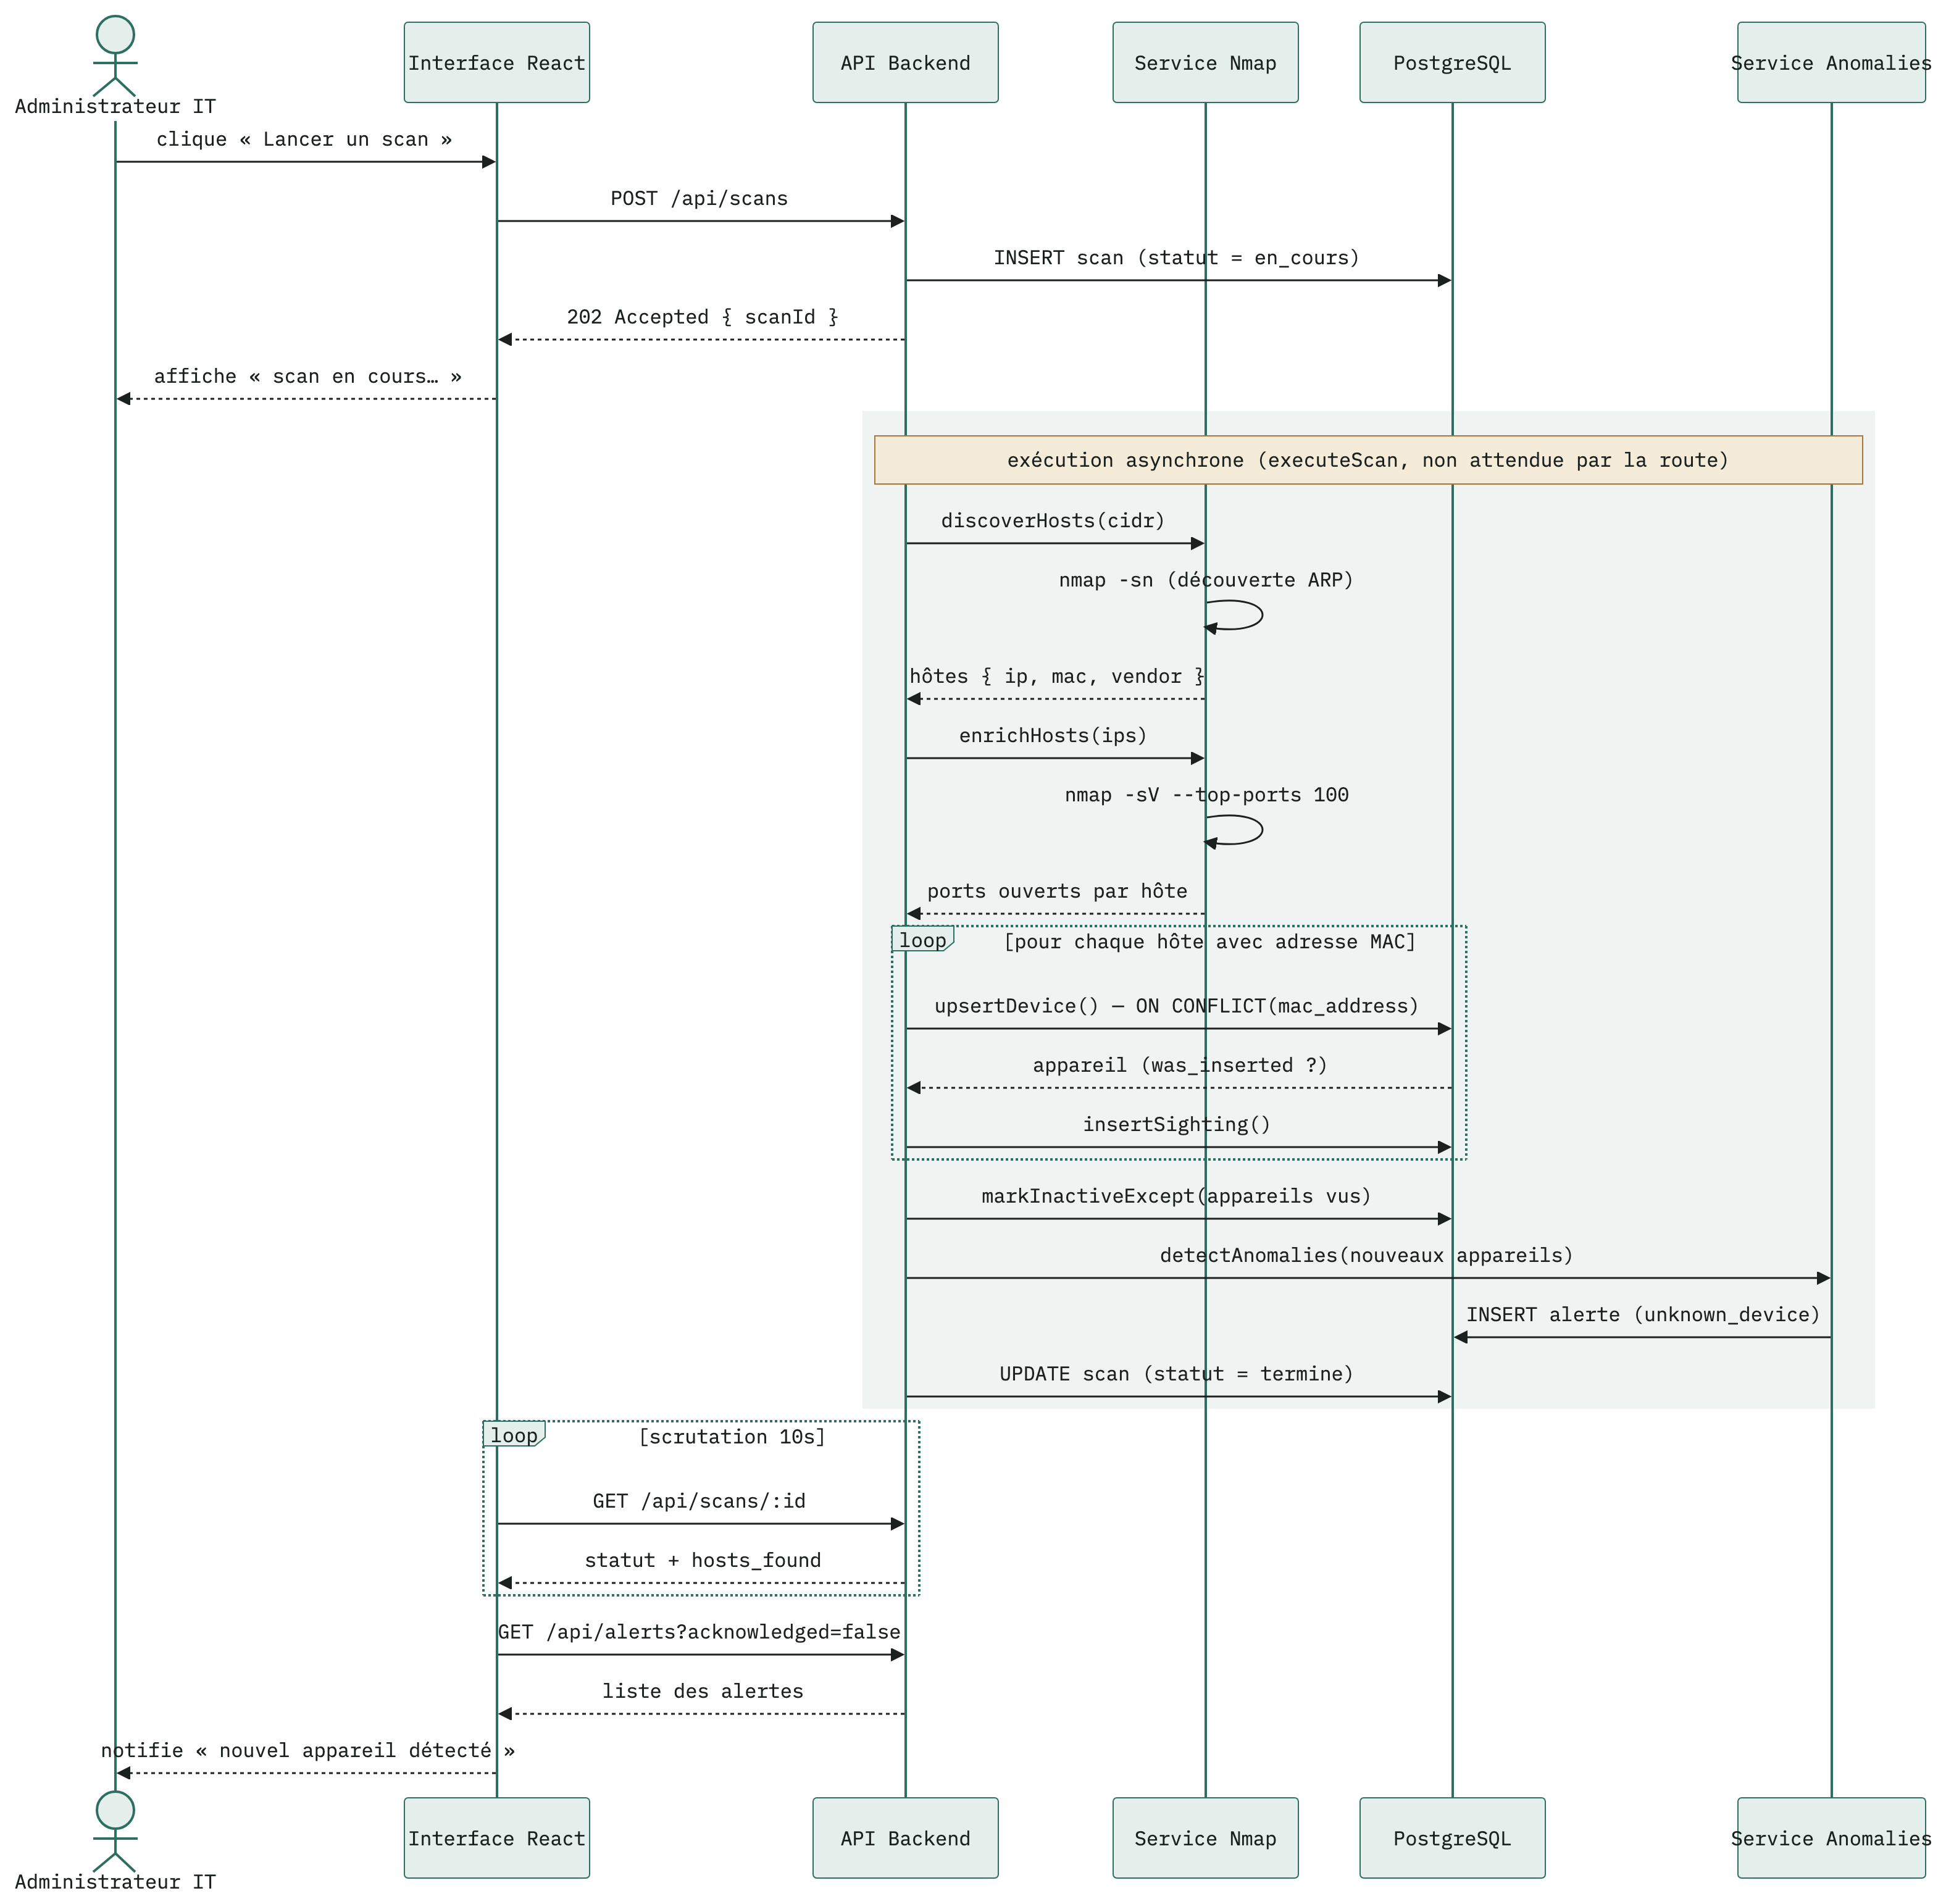
\includegraphics[width=0.85\textwidth]{figuresChapitres/diagramme_sequence.png}
    \caption{Diagramme de séquence -- exécution d'un scan et détection d'une anomalie}
    \label{fig:sequence}
\end{figure}

Le déclenchement d'un scan (\texttt{POST /api/scans}) répond immédiatement (\texttt{202
Accepted}) sans attendre la fin de l'exécution, qui se poursuit de façon asynchrone :
découverte des hôtes actifs par ARP (\texttt{nmap -sn}), puis enrichissement des hôtes
découverts par une énumération de ports (\texttt{nmap -sV --top-ports 100}). Pour chaque
équipement détecté possédant une adresse MAC, le backend met à jour la table des
équipements (\texttt{upsertDevice}, avec détection d'insertion via
\texttt{ON CONFLICT}) et journalise l'observation (\texttt{insertSighting}) ; les
équipements non revus lors du scan sont marqués inactifs, et le service d'anomalies
génère une alerte pour tout équipement nouvellement inséré. L'interface React scrute
ensuite périodiquement (\textit{polling} toutes les 10 secondes) le statut du scan et la
liste des alertes non acquittées.

\section{Modélisation des données (MCD)}

Le modèle conceptuel de données de la figure~\ref{fig:mcd} définit les entités et
relations utilisées pour stocker l'historique des équipements détectés, conformément au
schéma implémenté dans PostgreSQL.

\begin{figure}[H]
    \centering
    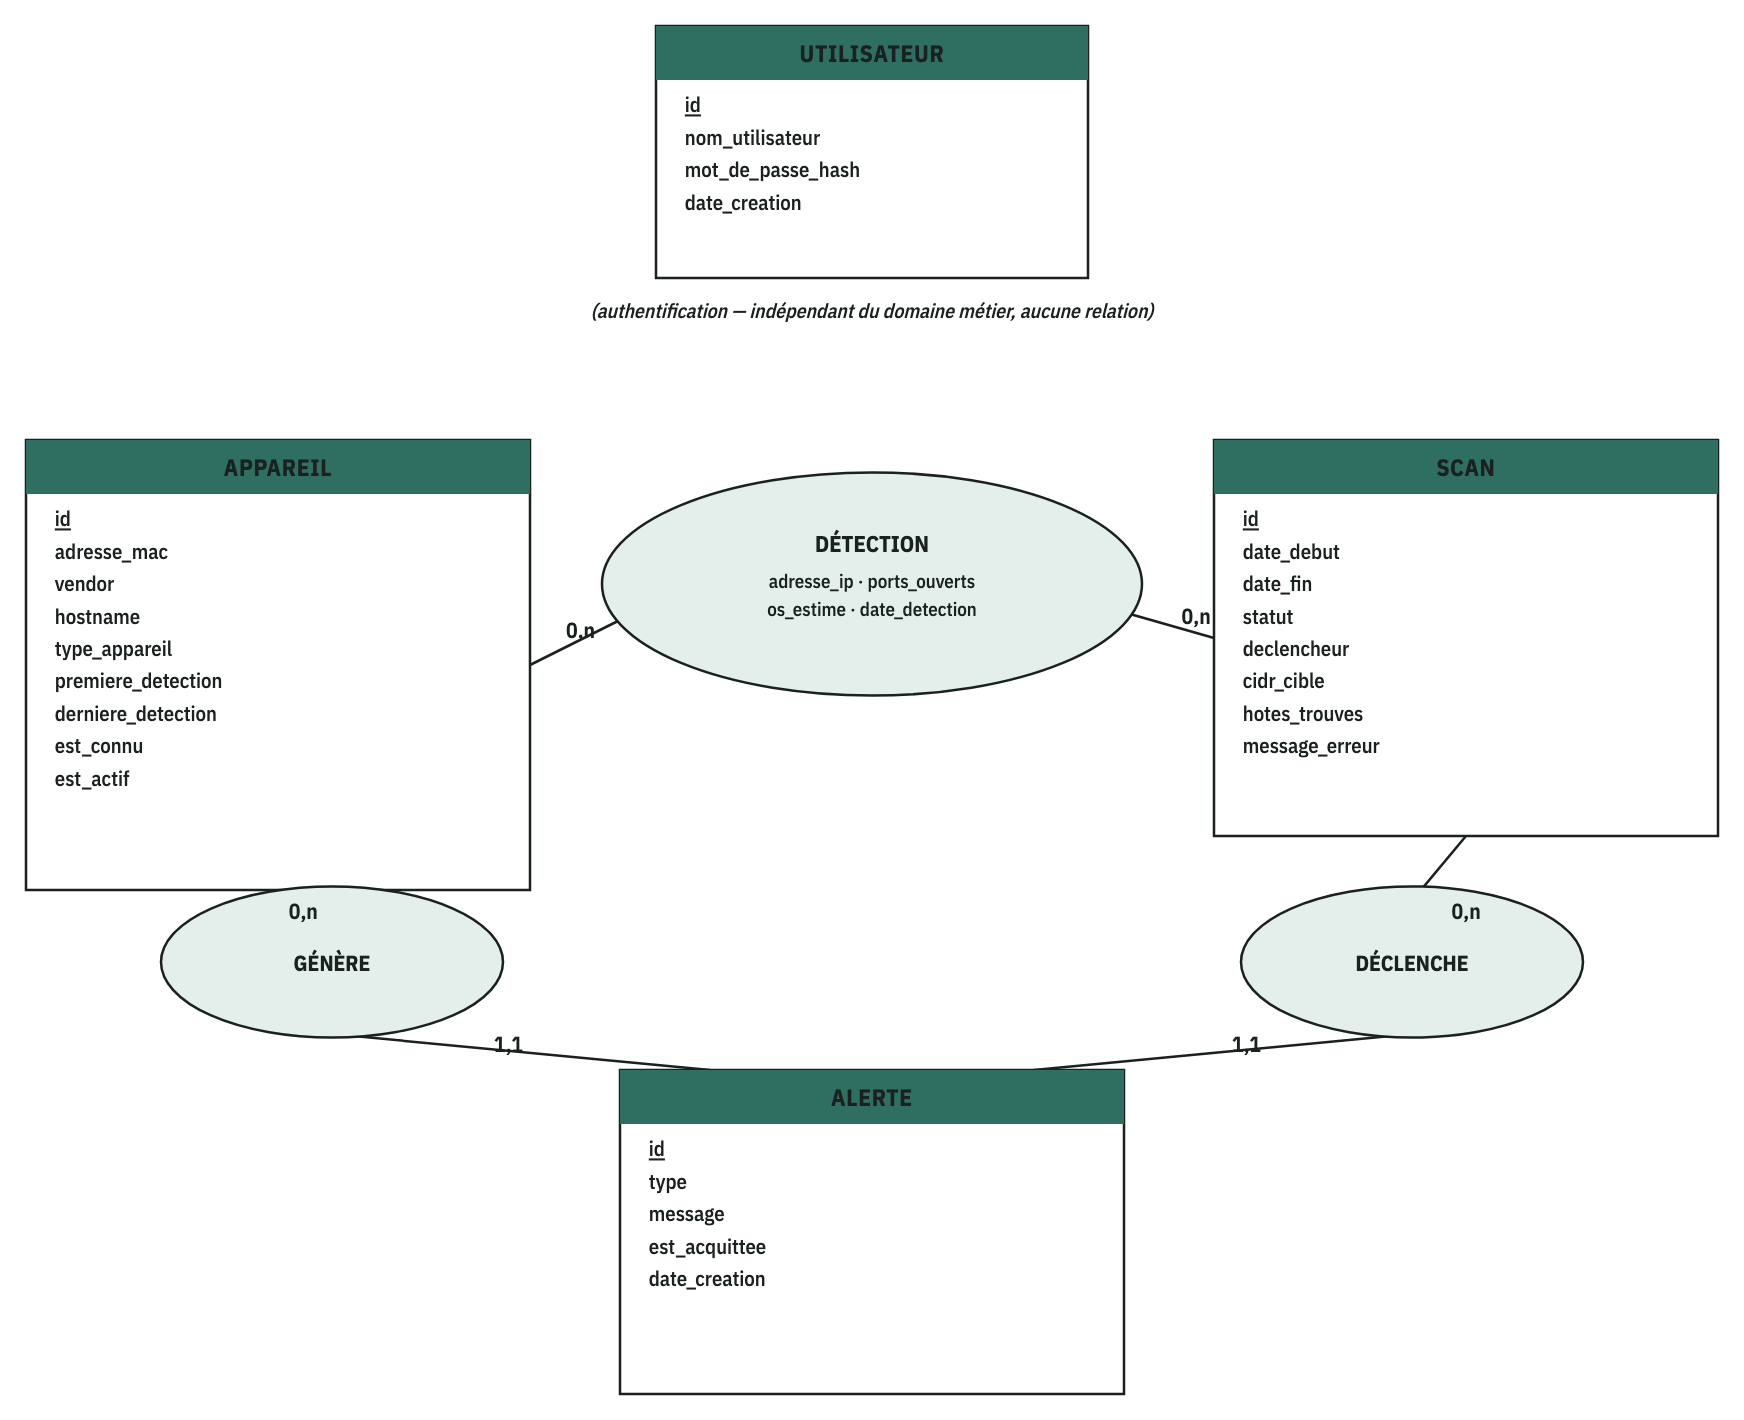
\includegraphics[width=0.8\textwidth]{figuresChapitres/mcd.png}
    \caption{Modèle conceptuel de données (MCD) de NetSentry}
    \label{fig:mcd}
\end{figure}

Le modèle distingue quatre entités principales. L'entité \textbf{APPAREIL} représente un
équipement, identifié par son adresse MAC -- stable dans le temps, contrairement à
l'adresse IP attribuée par DHCP -- et porte son statut courant (\texttt{est\_connu},
\texttt{est\_actif}). L'entité \textbf{SCAN} représente une exécution du moteur de scan
(manuelle ou planifiée), avec son statut et sa cible (CIDR). L'association
\textbf{DÉTECTION}, de cardinalité (0,n)--(0,n) entre \texttt{APPAREIL} et
\texttt{SCAN}, constitue l'historique append-only consultable dans le tableau de bord :
chaque détection porte l'adresse IP observée, les ports ouverts et la date de détection
pour cette occurrence précise du scan. L'entité \textbf{ALERTE} est générée soit par la
détection d'un nouvel appareil (association \textbf{GÉNÈRE}), soit par le scan qui l'a
révélée (association \textbf{DÉCLENCHE}), et peut être acquittée par l'administrateur
IT. Enfin, l'entité \textbf{UTILISATEUR}, dédiée à l'authentification, reste
indépendante du domaine métier et n'entretient aucune relation avec les autres entités.

\section{Conclusion}

Ce chapitre a permis de formaliser les interactions et les données du système
NetSentry à travers trois diagrammes complémentaires. Le chapitre suivant détaille
l'architecture technique retenue, les technologies mobilisées -- au premier rang
desquelles Nmap -- ainsi que l'organisation du travail durant le stage.
